\subsection{Forberedelses fasen}
I forberedelses fasen begyndte vi vores projektarbejde med selv at undersøge hvad diabetes er, og hvad det ville sige at leve med diabetes. Vi begyndte derefter at kigge på hvilke funktioner, som min sundhedsplatform havde, og hvilke siden manglede, som vi kunne forestille os ville styrke den. Vi kom frem til fire ideer - receptfornyelse, læring og videnscenter, socialt samlingssted og en forberedelse af siden til fremtidens teknologi. Gennem et interview og en spørgeskemaundersøgelse kom vi frem til,, at siden kunne forbedres ved at samle funktioner fra andre af sundhedsvæsenets sider, såsom receptfornyelse, og gøre dem tilgængelige på min sundhedsplatform. Ligeledes fandt vi også frem til, at brugerne af siden ofte ikke finder frem til den information, de søger, og der kunne derfor også samles mere information omkring diabetes på siden.\\
Nøgleordene for, at projektet kan lykkes, er brugervenlighed, tilgængelighed og udbredelse af kendskab til siden. Vi fandt, at mange af vores adspurgte diabetikere ikke kendte til siden, og dem som gjorde, var i mange forskellige aldre. Det er derfor vigtigt for projektet, at alle kan benytte de funktioner, som vil kunne findes på siden, og at brugervenligheden derfor i høj grad er i fokus.\\
Fra vores strategianalyse fandt vi, at det er vigtigt med sikre og intuitive løsninger, som brugeren selv kan benytte. Der er behov for et samlet system således, at brugeren selv kan finde al den nødvendige information. Samtidigt skal løsningerne være afprøvede og testet i drift, og de skal kunne udvides i fremtiden.
\begin{figure}[H]
	\centering
	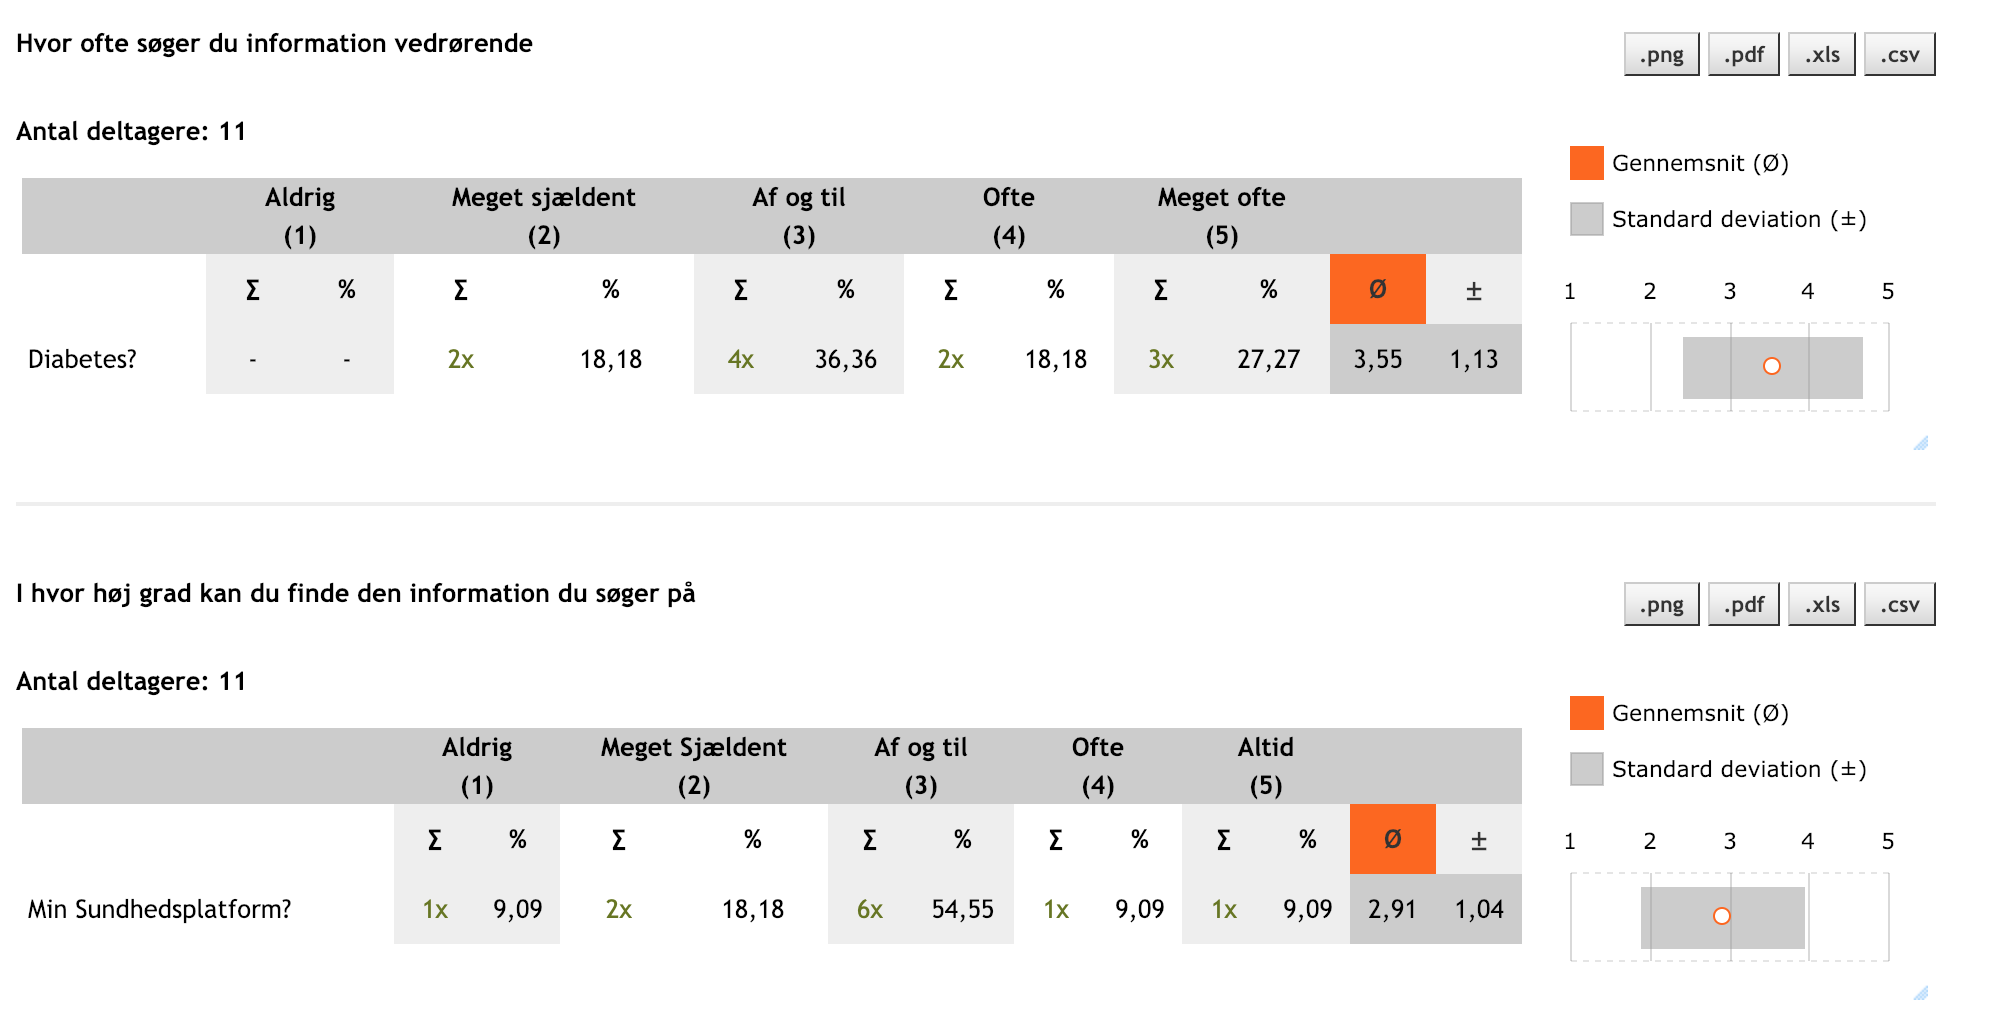
\includegraphics[width=\textwidth]{Materials/SeekingInformation}
	\caption{Svarfordeling på spørgsmål om søgning af information.}
\end{figure}
